%!TEX root = ../../super_main.tex

\section{Multi Project Organization}
\label{sec:multi_project_organization}

This semester project is the continuation of a widely spanning multi project with more than 50 developers which are organized in roughly 15 smaller groups, up to four developers per group, including a group consisting of the authors of this report. The multi project was split into three different project areas: \emph{Build and Deployment}, \emph{GUI}, \emph{Database}.

\todo{DONE-start}\subsection{Project areas}
The sub projects each have responsibilities for different parts of the project. The sub project \emph{Build and Deployment} is responsible for making the life easier for developers by improving and maintaining the work enviroment. This project is also responsible for making the products available to the customers.
\\\\
The project area \emph{GUI} short for (graphical user interface), which our group is a part of, is responsible for creating the applications, and developing the frontend of the entire \giraf software suite. For this reasons this sub project produce the facade to the customers and users of \giraf.
\\\\
The last area is the \emph{Database} sub project whcih is responsible for developing the backend of the system. This project should ensure that data can be stored and loaded consistently and persistently regardless of device. The \giraf system contains both remote storages but also local storages where the software suite is installed. This group is also responsible for maintaining consistency in between these storages.
\todo{DONE-end}

\subsection{Organization}
The multi project was organized using the process management method, Scrum \parencite{scrum}, more specific Scrum of Scrums. This method allows the groups in the multiproject to be self-organized, and enforces the individual groups to do work more independently. This independent work method fits great in since the individual groups are used to work in smaller projects groups. During the semester, the groups will acquire experience in working on a larger scale projects than previously encountered.
\\\\
As seen in \figref{fig:scrum_of_scrums} the Scrum of Scrums is split into three levels. The bottom most level is the individual groups, which work exactly as an ordinary development group using the Scrum method \todo{This sentence is incorrect. The individual groups decide for themselves. Do not write ordinary <-- marhlderfix}. The middle layer contains the three project areas where representatives from each individual group meet and synchronize their work at least twice a week. The top layer in \figref{fig:scrum_of_scrums} contains representatives from all of the project areas. Since stand-up meetings only occur once a week, it is important that every group sends a Scrum representative to join the meetings.

\begin{figure}[!htbp]
  \centering
    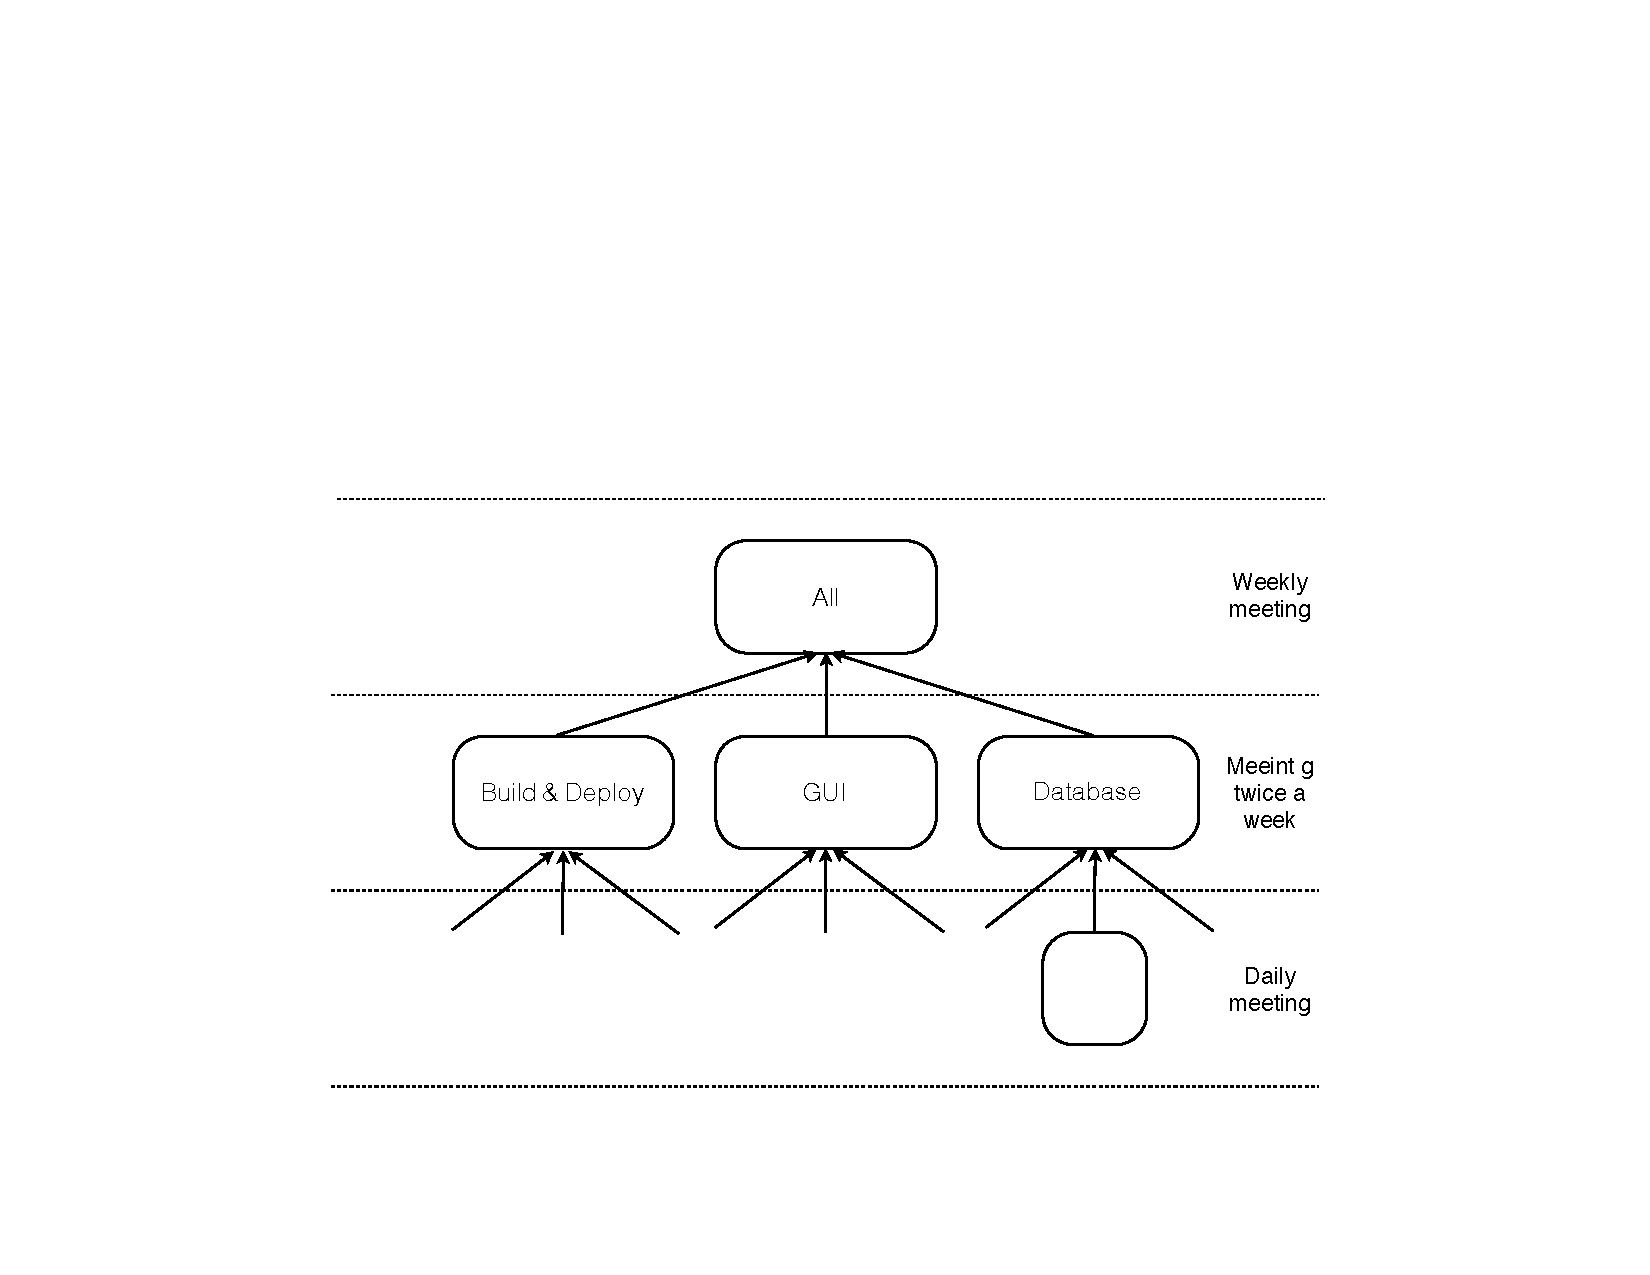
\includegraphics[width=0.8\textwidth]{scrum_of_scrums}
    \caption{Organization in Scrum of Scrums and meeting frequencies}
    \label{fig:scrum_of_scrums}
\end{figure}

\subsection{Roles and Responsibilities}
Several different roles and responsibilities were divided among the project groups. This group volunteered as ``Webadmin'' for the website at \url{http://giraf.cs.aau.dk/}. The ``Webadmin'' responsibility included administration of the official \giraf web page. Because one of the members had previous experience with Android, he was appointed as ``Android Guru''. His responsibility included helping out with Android related issues that groups could not handle within reasonable time themselves and setting up a general Android guideline.

\subsection{Further Reading}
For further description of the \giraf Development method we refer to the description made by group SW609F15 in their report\footnote{This report has not yet been published, and we are therefore unable to cite it properly}.